\subsection{Auflösungsvermögen}
\label{sec:aufloesea}

Die beiden benachbarten Störstellen 1, 2, vgl. Abbildung \ref{fig:acrylblock},
wurden mit allen drei verfügbaren Sonden vermessen,
die Messwerte stehen in Tabelle \ref{tab:aufloesung}.
Die Abbildung \ref{fig:aufloesung} zeigt die A-Scans von Ultraschallsonden
mit unterschiedlichen Frequenzen. Die Achse zeigt die Tiefe in $\si{\milli\meter}$.

\begin{figure}
    \centering
    \begin{subfigure}{0.2\textwidth}
        \centering
        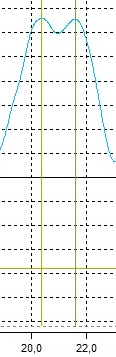
\includegraphics[height=7cm]{content/bilder/a-scan-blau.jpg}
        \caption{$\SI{1}{\mega\hertz}$ - (blau)}
        \label{fig:1mhz}
    \end{subfigure}
    \begin{subfigure}{0.2\textwidth}
        \centering
        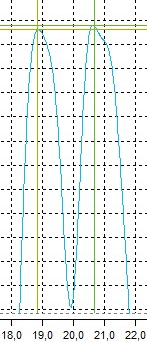
\includegraphics[height=7cm]{content/bilder/a-scan-rot.jpg}
        \caption{$\SI{2}{\mega\hertz}$ - (rot)}
        \label{fig:2mhz}
    \end{subfigure}
    \begin{subfigure}{0.5\textwidth}
        \centering
        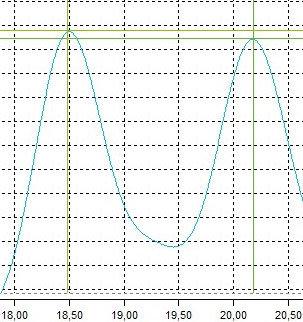
\includegraphics[height=7cm]{content/bilder/a-scan-gruen.jpg}
        \caption{$\SI{4}{\mega\hertz}$ - (grün)}
        \label{fig:4mhz}
    \end{subfigure}
    \caption{Scans der jeweiligen Sonde.}
    \label{fig:aufloesung}
\end{figure}

\begin{table}
    \centering
    \caption{Messwerte der Auflösungs-Messung.}
    \label{tab:aufloesung}
    \begin{tabular}{c S[table-format=1.0]
        S[table-format=2.2] S[table-format=2.2]
        S[table-format=1.3] S[table-format=1.3]}
        \toprule
        {Farbe}
        & {$ν\:/\:\si{\mega\hertz}$}
        & {$h_1\:/\:\si{\milli\meter}$}
        & {$h_2\:/\:\si{\milli\meter}$}
        & {$A_1\:/\:\si{\volt}$}
        & {$A_2\:/\:\si{\volt}$}\\
        \midrule
        blau & 1 & 20.38 & 21.62 & 0.663 & 0.658 \\
        rot  & 2 & 18.82 & 20.66 & 1.233 & 1.242 \\
        grün & 4 & 18.49 & 20.18 & 0.294 & 0.286 \\
        \bottomrule
    \end{tabular}
\end{table}
